%-----------------------------------
% Define document and include general packages
%-----------------------------------
\documentclass[12pt,oneside,titlepage,listof=totoc,bibliography=totoc]{scrartcl}
\usepackage[utf8]{inputenc}
\usepackage[ngerman]{babel}
\usepackage[babel,german=quotes]{csquotes}
\usepackage[T1]{fontenc}
\usepackage{fancyhdr}
\usepackage{fancybox}
\usepackage[a4paper, left=4cm, right=2cm, top=3cm, bottom=2cm]{geometry}
\usepackage{graphicx}
\usepackage{colortbl}
\usepackage{array}
\usepackage{float}      %Positionierung von Abb. und Tabellen mit [H] erzwingen
\usepackage{footnote}
\usepackage{caption}
\usepackage{mdwlist}
\usepackage{amssymb}
\usepackage{mathptmx}
\usepackage{amsmath}
\usepackage[table]{xcolor}
\usepackage{marvosym}			% Verwendung von Symbolen, z.B. perfektes Eurozeichen
\usepackage[colorlinks=true,linkcolor=black]{hyperref}
\definecolor{darkblack}{rgb}{0,0,0}
\hypersetup{colorlinks=true, breaklinks=true, linkcolor=darkblack, menucolor=darkblack, urlcolor=darkblack}
\usepackage{times}
\fontfamily{ptm}\selectfont

% Mehrere Fussnoten nacheinander mit Komma separiert
\usepackage[multiple]{footmisc}
% todo Aufgaben als Kommentare verfassen für verschiedene Editoren
\usepackage{todonotes}

%Pakete für Tabellen
\usepackage{epstopdf}
\usepackage{nicefrac} % Brüche
\usepackage{multirow}
\usepackage{rotating} % vertikal schreiben
\usepackage{colortbl}
\usepackage{mdwlist}

\definecolor{dunkelgrau}{rgb}{0.8,0.8,0.8}
\definecolor{hellgrau}{rgb}{0.0,0.7,0.99}
% Colors for listings
\definecolor{mauve}{rgb}{0.58,0,0.82}
\definecolor{dkgreen}{rgb}{0,0.6,0}

% sauber formatierter Quelltext
\usepackage{listings}
\lstset{numbers=left,
	numberstyle=\tiny,
	numbersep=5pt,
	breaklines=true,
	showstringspaces=false,
	frame=l ,
	xleftmargin=5pt,
	xrightmargin=5pt,
	basicstyle=\ttfamily\scriptsize,
	stepnumber=1,
	keywordstyle=\color{blue},          % keyword style
  	commentstyle=\color{dkgreen},       % comment style
  	stringstyle=\color{mauve}         % string literal style
}

% Biblatex
\usepackage[
backend=bibtex,
style=numeric,
citestyle=authoryear-ibid,
bibstyle=authoryear,
ibidpage=true, %siehe Doku
pagetracker=false, %ebd
url=false,
isbn=false,
notetype=footonly,
hyperref=false,
sortlocale=de]{biblatex}

%weitere Anpassungen für BibLaTex
% Opptionen für Biblatex
\ExecuteBibliographyOptions{%
giveninits=false,
isbn=true, 
url=true, 
doi=false, 
eprint=false,
maxbibnames=7, % Alle Autoren (kein et al.)
maxcitenames=2, % et al. ab dem 3. Autor
backref=false, % Rückverweise auf Zitatseiten
bibencoding=utf8, % wenn .bib in utf8, sonst ascii
bibwarn=true, % Warnung bei fehlerhafter bib-Datei
}%

% et al. an Stelle von u.a.
\DefineBibliographyStrings{ngerman}{ 
   andothers = {{et\,al\adddot}},             
}

% Klammern um das Jahr in der Fußnote
\renewbibmacro*{cite:labelyear+extrayear}{% 
  \iffieldundef{labelyear} 
    {} 
    {\printtext[bibhyperref]{% 
       \mkbibparens{% 
         \printfield{labelyear}% 
         \printfield{extrayear}}}}}

\DeclareNameFormat{last-first}{%
  \iffirstinits
    {\usebibmacro{name:family-given}
        {\namepartfamily}
        {\namepartgiveni}
        {\namepartprefix}
        {\namepartsuffix}
    }
    {\usebibmacro{name:family-given}
        {\namepartfamily}
        {\namepartgiven}
        {\namepartprefix}
        {\namepartsuffix}
    }%
  \usebibmacro{name:andothers}}

% Alternative Notation der Fußnoten 
% Zeigt sowohl den Nachnamen als auch den Vornamen an
% Beispiel: \fullfootcite[Vgl. ][Seite 5]{Tanenbaum.2003} 
\DeclareCiteCommand{\fullfootcite}[\mkbibfootnote]
  {\usebibmacro{prenote}}
  {\usebibmacro{citeindex}%
    \printnames[sortname][1-1]{author}%
    \addspace (\printfield{year})}
  {\addsemicolon\space}
  {\usebibmacro{postnote}}

%Autoren (Nachname, Vorname)
\DeclareNameAlias{default}{family-given}

%Reihenfolge von publisher, year, address verändern
% Achtung, bisher nur für den Typ @book definiert

%% Definiert @Book Eintrag
\DeclareBibliographyDriver{book}{%
  \printnames{author}%
  \setunit*{\space (}%
  \printfield{year}\setunit*{):\space}%
  \printfield{title}%
  \setunit*{,\space}%
  \printfield{edition}%
  \setunit*{\addcomma\space}%
  \printlist{publisher}%
  \newunit\newblockpunct
  \printlist{location}%
  \setunit*{\space}%
  \printfield{year}%
  \setunit*{,\space}% 
  \printfield{isbn}%
  \finentry}

%% Definiert @Online Eintrag
\DeclareBibliographyDriver{online}{%
  \printnames{author}%
  \newunit\newblockpunct
  \printfield{title}%
  \setunit*{,\space}%
  %\newunit\newblock
  \printfield{url}%
  \setunit*{,\space}%
  \printfield{note}%
  \finentry}
  
%% Definiert @Article Eintrag
\DeclareBibliographyDriver{article}{%
  \printnames{author}%
  \setunit*{\space (}%
  \printfield{year}\setunit*{):\space}%
  \newblockpunct
  \printfield{title}%
  \setunit*{.\space In:\space}%
  %\newunit\newblock
  \usebibmacro{journal}%
  \setunit*{,\space}%
  \printfield{volume}\newunit{ Jg.}%
  \setunit*{,\space Heft Nr.\space}%
  \printfield{number}%
  \setunit*{,\space}%
  \printfield{pages}%
  \finentry}  
  
\DeclareBibliographyDriver{legislation}{%
  \usebibmacro{bibindex}%
  \usebibmacro{begentry}%
  \usebibmacro{title}%
  \setunit{\space}%
  \printfield{note}%
  \usebibmacro{pageref}%
  \usebibmacro{finentry}}

%Doppelpunkt nach dem letzten Autor
\renewcommand*{\labelnamepunct}{\addcolon\addspace }

%Komma an Stelle des Punktes
\renewcommand*{\newunitpunct}{\addcomma\space}

%Autoren durch Semikolon trennen
\newcommand*{\bibmultinamedelim}{\addsemicolon\space}% 
\newcommand*{\bibfinalnamedelim}{\addsemicolon\space}% 
\AtBeginBibliography{% 
  \let\multinamedelim\bibmultinamedelim 
  \let\finalnamedelim\bibfinalnamedelim 
}

%Titel nicht kursiv anzeigen 
\DeclareFieldFormat{title}{#1\isdot}



%Bib-Datei einbinden
\addbibresource{literatur/literatur.bib}

% Pfad fuer Abbildungen
\graphicspath{{./}{./abbildungen/}}

%-----------------------------------
% Weitere Ebene einfügen
\usepackage{titletoc}

\makeatletter

% Setze die Tiefe des Inhaltsverzeichnis auf 4 Ebenen
% Damit erscheinen \paragraph-Sektionen auch im Inhaltsverzeichnis
\setcounter{secnumdepth}{4}
\setcounter{tocdepth}{4}

% Fuege Abstand nach unten wie in einer normalen \section hinzu
% Andernfalls haette \paragraph keinen Zeilenumbruch
% Der Zeilenumbruch koennte mit einer leeren \mbox{} ersetzt werden
% Jedoch klebt dann der Text relativ nah an der Ueberschrift
\renewcommand{\paragraph}{%
  \@startsection{paragraph}{4}%
  {\z@}{3.25ex \@plus 1ex \@minus .2ex}{1.5ex plus 0.2ex}%
  {\normalfont\normalsize\bfseries\sffamily}%
}

\makeatother


%-----------------------------------
% Zeilenabstand 1,5-zeilig
%-----------------------------------
\usepackage{setspace}
\onehalfspacing

%-----------------------------------
% Absätze durch eine neue Zeile
%-----------------------------------
\setlength{\parindent}{0mm}
\setlength{\parskip}{0.8em plus 0.5em minus 0.3em}

\sloppy					%Abstände variieren
\pagestyle{headings}

%-----------------------------------
% Abkürzungsverzeichnis
%-----------------------------------
\usepackage[intoc]{nomencl}
\renewcommand{\nomname}{Abkürzungsverzeichnis}
\setlength{\nomlabelwidth}{.20\textwidth}
\renewcommand{\nomlabel}[1]{#1 \dotfill}
\setlength{\nomitemsep}{-\parsep}
\makenomenclature

%-----------------------------------
% Meta informationen
%-----------------------------------
%-----------------------------------
% Meta Informationen zur Arbeit
%-----------------------------------

% Autor
\newcommand{\myAutor}{Aleksandar Simic}

% Adresse
\newcommand{\myAdresse}{Stüvestraße 34 \\ \> \> 45144 Essen}

% Titel der Arbeit
\newcommand{\myTitel}{Einführung eines Smart Workplace in einem mittelständischen Unternehmen unter Berücksichtigung der rechtlichen Grundlagen der Arbeitsplatzergonomie}

% Betreuer
\newcommand{\myBetreuer}{Dipl.-Wirtschaftsinf. Mike Heuser}

% Lehrveranstaltung
\newcommand{\myLehrveranstaltung}{IT-Infrastruktur}

% Matrikelnummer
\newcommand{\myMatrikelNr}{396631}

% Ort
\newcommand{\myOrt}{Essen}

% Datum der Abgabe
\newcommand{\myAbgabeDatum}{25. Juni 2017}

% Semesterzahl
\newcommand{\mySemesterZahl}{4}

% Name der Hochschule
\newcommand{\myHochschulName}{FOM Hochschule für Oekonomie \& Management Essen}

% Standort der Hochschule
\newcommand{\myHochschulStandort}{Standort Essen}

% Studiengang
\newcommand{\myStudiengang}{Wirtschaftsinformatik}

% Firma
\newcommand{\myFirma}{GFOS mbH}

%-----------------------------------
% Kopfbereich / Header definieren
%-----------------------------------
\pagestyle{fancy}
\fancyhf{}
\fancyhead[R]{\thepage}								% Seitenzahl oben, rechts
%\fancyhead[L]{\leftmark}							% kein Footer vorhanden
\renewcommand{\headrulewidth}{0.4pt}

\makeindex % <=== !!!!!

%-----------------------------------
% Start the document here:
%-----------------------------------
\begin{document}

\pagenumbering{Roman}								% Seitennumerierung auf römisch umstellen
\renewcommand{\refname}{Literaturverzeichnis}		% "Literatur" in
%"Literaturverzeichnis" umbenennen
\newcolumntype{C}{>{\centering\arraybackslash}X}	% Neuer Tabellen-Spalten-Typ:
%Zentriert und umbrechbar

%-----------------------------------
% Titlepage
%-----------------------------------
\begin{titlepage}
	\newgeometry{left=2cm, right=2cm, top=2cm, bottom=2cm}
	\begin{center}
		\textbf{\myHochschulName}\\
		\textbf{\myHochschulStandort}\\
		\vspace{1.5cm}
			
\includegraphics[width=3cm]{abbildungen/fomLogo.jpg} \\
		\vspace{1.5cm}
		Berufsbegleitender Studiengang\\
		\myStudiengang, \mySemesterZahl. Semester\\
		\vspace{2cm}
		\textbf{Hausarbeit im Rahmen der Lehrveranstaltung}\\
		\textbf{\myLehrveranstaltung}\\
		\vspace{2cm}
		über das Thema\\
		\Huge{\myTitel}\\
		\vspace{0.2cm}
	\end{center}
	\normalsize
	\vfill
	\begin{tabbing}
		Links \= Mitte \= Rechts\kill

		Autor: \> \> \myAutor\\
		\> \>  Matrikelnr.: \myMatrikelNr\\
		\> \> \myAdresse\\
		\> \> \\
		Abgabe: \> \> \myAbgabeDatum
	\end{tabbing}
\end{titlepage}

%-------Ende Titelseite-------------

%-----------------------------------
% Sperrvermerk
%-----------------------------------
%\input{kapitel/anhang/sperrvermerk}

%-----------------------------------
% Inhaltsverzeichnis
%-----------------------------------
\setcounter{page}{2}
\tableofcontents
\newpage

%-----------------------------------
% Abbildungsverzeichnis
%-----------------------------------
\listoffigures
\newpage

%-----------------------------------
% Abkürzungsverzeichnis
%-----------------------------------
\printnomenclature
\newpage

%-----------------------------------
% Seitennummerierung auf arabisch und ab 1 beginnend umstellen
%-----------------------------------
\pagenumbering{arabic}
\setcounter{page}{1}
%-----------------------------------
% Kapitel / Inhalte
%-----------------------------------
\section{Einleitung}
\subsection{Themenvorstellung}
In der heutigen Zeit tendieren Unternehmen vermehrt dazu, zur Vereinfachung und Prozessoptimierung neue Technologien in den Arbeitsalltag einfließen zu lassen. Dies hat ebenfalls einen Einfluss auf die Arbeitsumgebungen der Mitarbeiter, die standardmäßigen Büros mit Arbeitsplatzrechnern weichen den Großräumen mit mobilen Endgeräten. Zuletzt hat das Unternehmen Microsoft in seinem münchener Standort so eine intelligente Arbeitsumgebung, auch Smart Workplace oder Smart Workspace genannt, eingerichtet\footcite[Vgl.][]{MicrosoftArtikel}. Diese moderne Entwicklung ist die Motivation hinter dieser Seminararbeit.

\subsection{Zielsetzung}
Im Folgenden steht die Darstellung eines Smart Workplace und dessen mögliche Umsetzungen im Vordergrund. Es sollen Anwendungsfälle für ein mittelständisches Unternehmen und die dafür notwendigen Voraussetzungen vorgestellt werden. Auch eventuelle Konflikte mit aktuellen gesetzlichen Verordnungen bezüglich der Arbeitspaltzergonomie werden eruiert und versucht mit dem Einsatz neuer Technologien in Einklang zu bringen.

\subsection{Aufbau}
Beginnend wird der Begriff des Smart Workplace näher definiert und erläutert. Anschließend werden die einsetzbaren Technologien und räumlichen Gestaltungsmöglichkeiten dargestellt und gleichzeitig die Voraussetzungen für deren Umsetzung gepüft. Die Einführung der Systeme wird schrittweise dargelegt. Sollten bezüglich des Einsatzes der Technologien oder der Raumgestaltung Konflikte mit den rechtlichen Grundlagen zur Arbeitsplatzergonomie existieren, werden diese aufgezeigt und mögliche Gesetzesanpassungen präsentiert um die Nutzung zukünfitig zu ermöglichen. Abschließend wird die Arbeit in einem Fazit reflektiert und die wesentlichen inhaltlichen Aspekte zusammengefasst.
\newpage
\section{Analyse}
\subsection{Konzeption}
Zunächst gilt es die allgemeinen Grundbegriffe zu definieren, beginnend mit dem Begriff der Datenbanken. Dies sind organisierte Anordnungen von Daten bzw. Informationen auf einem Computersystem, welches zum Speichern und Abfragen von Informationen geeignet ist. Die Art der Anordnung hängt von dem jeweligen Datenbankmodell ab. In einem relationalen Datenbankmodell, von welchem im weiteren Verlauf der Arbeit ausgegangen wird, besteht eine Datenbank aus mindestens einer oder mehreren miteinander in Verbindung stehenden Tabellen. Diese enthalten die gespeicherten Informationen in Form von Zeilen und Spalten, wobei die Spalten eine Informationsart darstellen und eine Zeile die Daten zu jeder Spalte enthält.
Um diese Daten verwalten zu können, werden vom \nomenclature{DBMS}{Datenbankmanagementsystem}Datenbankmanagementsystem (DBMS) eine Reihe von Ressourcen zur Verfügung gestellt.\footcite[Vgl.][]{samu2002database}

Dabei wird weitestgehend die Unabhängigkeit der Datenrepräsentation von Optimierung und Änderung der Speicherstrukturen durch das Prinzip der Datenunabhängigkeit garantiert\footcite[Vgl.][Seite 1]{saake2011datenbanken}.

\subsection{Zuständigkeitsbestimmung}
Structured Query Language (SQL) \nomenclature{SQL}{Structured Query Language}ist eine nicht-prozedurale Sprache, welche in den meisten relationalen Datenbanken geläufig ist. Sie wird sowohl von der Datenbank zur internen Selbstverwaltung als auch von Benutzern verwendet, um die dort gespeicherten Daten zu manipulieren und abzufragen. Außerdem lässt sich mit SQL Befehlen zum Beispiel zwischen verschiedenen Datenbanksystemen bewegen und Abfragen generieren welche in der Benutzeroberfläche so nicht repräsentiert werden oder zur Performanceanalyse genutzt werden können.\footcite[Vgl.][]{UniversityofDelaware}

Es handelt sich hierbei um eine dem Englischen ähnliche Sprache. Sie wurde 1974 von der International Business Machines Corp. (IBM) \nomenclature{IBM}{International Business Machines}erfunden, wird stetig erweitert und ist mittlerweile de-facto weltweiter Standard. Bestehend aus rund 60 Befehlen lässt sie sich auf fast jedem Computersystem ausführen.\footcite[Vgl.][]{BusinessDictionary}
Die am häufigsten anzutreffenden Befehle sind SELECT, INSERT, UPDATE, CREATE, UNION SELECT und DELETE\footcite[Vgl.][Seite 486]{OlearySteele}.
Diese Befehle gehören zur Data Definition Language (DDL)\nomenclature{DDL}{Data Definition Language}, welche zur Definition oder Anpassung von Datenbankstrukturen genutzt wird. Befehle, welche Daten selbst selektieren oder ändern wie INSERT, UPDATE oder DELETE gehören der Data Manipulation Language (DML) \nomenclature{DML}{Data Manipulation Language}an.\footcite[Vgl.][]{UniversityofDelaware}

\subsection{Teambildung}
Procedural Language / Structured Query Language (PL/SQL)\nomenclature{PL/SQL}{Procedural Language / Structured Query Language}, die prozedurale Erweiterung von SQL durch Oracle, ist eine portable, high-performance Transaktionsverarbeitungssprache. Sie kombiniert die Datenmanipulationsfunktion von SQL mit der Verarbeitungsfunktion von prozeduralen Sprachen. In PL/SQL ist es wie in anderen prozeduralen Programmiersprachen ebenfalls möglich, Konstanten und Variablen zu deklarieren, Laufzeitfehler aufzudecken und Unterprogramme zu definieren.\footcite[Vgl.][Seite 1-1 ff]{oracle}

\subsection{Aufgabenverteilung}
Da in dieser Arbeit nicht nur auf den allgemeinen Aufbau von Triggern, sondern auch auf die Spezialitäten auf Oracle Systemen eingegangen wird, gehört dies ebenfalls zu den Grundlagen.

Die Oracle Corporation ist ein IT-Dienstleistungsunternehmen, welches Datenbank- und Middleware-Softwarelösungen, Applikationssoftware und Computerhardware wie Server und Speichersysteme entwickelt, produziert, vermarktet und vertreibt. In diesem Bereich gehört Oracle zu den weltweit führenden Anbietern.\footcite[Vgl.][]{OracleCorp}

\subsection{Entwicklung}

\subsection{Qualitätssicherung}

\subsection{Abnahme}

\newpage
\section{Mögliche Aspekte}
\subsection{Persönliche mobile Arbeitsumgebung}
Heutzutage werden Computer für alle möglichen Tätigkeiten in der Arbeitswelt benötigt, ob nun für kleinere Aufgaben oder für komplexe Berechnung mit Hilfe eines am Netzwerk angeschlossenen Supercomputers. In einer modernen Umgebung kann es unter Umständen notwendig sein den Arbeitsplatz aufgrund einer Tätigkeit zu wechseln um diese ausführen zu können. Dies hat allerdings zur Folge, dass dort der eigene Rechner mit den zugehörigen Daten und möglicherweise auch die benötigte Rechenleistung nicht verfügbar ist.
Um für die Benutzer eine auf allen Rechnersystemen einheitliche Bedienerfahrung gewährleisten zu können, lässt sich eine sogenannte mobile personalisierte virtuelle Computerumgebung (MOVE)\nomenclature{MOVE}{Mobile Personalized Virtual Computing Environment} nutzen. Durch diese Umgebung wird dem Benutzer auf jeder beliebigen Maschine eine gleichmäßig konsistente Desktop-Rechner-Umgebung präsentiert, welche sowohl die gleichen personenbezogenen Daten und Software als auch die verfügbare Rechenleistung liefert wie am eigenen Arbeitsplatzrechner. Eine solche Desktop-Rechner-Umgebung besteht zum Großteil aus der installierten Software einschließlich des Betriebs- und Dateisystems. Diese könnten zwar vom Speichermedium auf ein anderes übertragen werden, aufgrund der engen Koppelung ließe sich diese allerdings nicht einfach auf einem neuen System ausführen. Um diese Abstraktion gewährleisten zu können, wird die Technologie der virtuellen Maschinen (VM)\nomenclature{VM}{Virtual Maschine} genutzt.\footcite[Vgl.][Seite 890 f.]{MOVE}

Bei der Virtualisierung werden mit Hilfe von Technologien die Ressourcen eines Rechnersystems auf mehrere einzelne Klienten aufgeteilt um diese effektiver und flexibler nutzbar zu machen. Dies geschieht dadurch, dass unterschiedliche Klassen von Anwendungen auf wenigen physischen Systemen konsolidiert und von mehreren unabhängigen Betriebssysteminstanzen gleichzeitig genutzt werden können.\footcite[Vgl.][Seite 197]{InformatikSpektrum} Diese Virtualisierung wird mit der Hypervisor Technologie implementiert. Ein Hypervisor, oder auch Virtual Maschine Monitor (VMM)\nomenclature{VMM}{Virtual Maschine Monitor} genannt, ist ein Stück Hardware oder Software welches Systemressourcen virtualisiert, wobei zwischen Typ 1 und Typ 2 Hypervisors unterschieden wird. Typ 1 Hypervisors sind direkt auf der Hardware implementiert, Typ 2 Hypervisors laufen dagegen auf einem Host Betriebssystem. Dieses stellt Dienste wie Speichermanagement zur Virtualisierung zur Verfügung.\footcite[Vgl.][]{ibm}

\begin{figure}[H]
\begin{center}
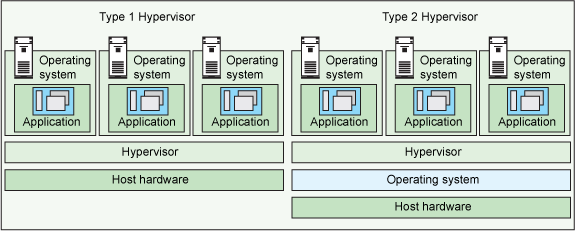
\includegraphics[width=0.9\textwidth]{hypervisors}
\caption{Unterschiede zwischen den Typ 1 und Typ 2 Hypervisors}
Quelle: \cite[]{ibm}
\end{center}
\end{figure}
\vspace{-1cm}
\newpage
\section{Rechtliche Grundlagen}
Vorgaben bezüglich der Gestaltung moderner Bildschirmarbeitsplätze sind in mehreren Gesetzen verankert. Schon 1996 wurde mit der BildschirmArbV (Bildschirmarbeitsverordnung)\nomenclature{BildschArbV}{Bildschirmarbeitsverordnung} allerdings eine speziell darauf bezogene Verordnung erlassen. Gemäß § 1 Abs. 2 gilt sie nicht für Bildschirmarbeitsplätze, die beweglich sind und nicht über einen längeren Zeitraum am gleichen Arbeitsplatz verwendet werden und für Geräte mit kleinem Bildschirm. Daher können Wearables trotz ihrer kleinen Bildschirme als primäre Arbeitsmittel genutzt werden.

Laptops hingegen können nur verwendet werden, wenn sich der Arbeitsplatz stetig wechselt, da sie in diesem Fall nicht von der BildschArbV betroffen sind. Im Anhang der BildschArbV werden die Anforderungen an Bildschirmgeräte, Tastaturen, sonstige Arbeitsmittel und die Arbeitsumgebung gestellt. Hier wird unter anderem in den Punkten 5-7 festgelegt, dass der Bildschirm frei dreh- und neigbar und die Tastatur vom Bildschirm getrennt sein muss. Da bei einem Laptop zumeist Bildschirm und Tastatur untrennbar voneinander sind, muss eine externe Tastatur am Laptop angeschlossen werden um eine Nutzung zu erlauben.

Die CGLX-Technologie kann für Meetings verwendet werden, da diese meist nicht lange dauern. Als fester Arbeitsplatz können sie allerdings nicht genutzt werden, weil kein ergonomisches Arbeiten mit einem Multi-Touch-Table und einer Leinwand möglich ist. Die Thin Clients der MOVE-Architektur müssen zur Verwendung die vorgeschriebene Ausstattung besitzen und die Bedingungen für eine gesunde Arbeitsumgebung wie eine Lichtschutzvorrichtung für die Fenster oder eine erträgliche Luftfeuchtigkeit müssen erfüllt sein, um das MOVE-System implementieren zu können.\nocite{BildschArbV}
\newpage
\section{Schlussbetrachtung}
\subsection{Fazit}

\subsection{Ausblick}

%-----------------------------------
% Literaturverzeichnis
%-----------------------------------
\newpage
%\addcontentsline{toc}{section}{Literatur}

\pagenumbering{Roman} %Zähler wieder römisch ausgeben
\setcounter{page}{5}  %Zähler manuell hochsetzen

%\printbibliography

% Alternative Darstellung:
% Literaturverzeichnis nach Typ (@book, @arcticle ...) sortiert.
% Dazu die Zeile (\printbibliography) auskommentieren und folgenden code verwenden:

\printbibheading
\printbibliography[type=article,heading=subbibliography,title={Zeitschriften}]
\printbibliography[type=book,heading=subbibliography,title={Bücher}]
\printbibliography[type=patent,heading=subbibliography,title={Patente}]
\printbibliography[type=online,heading=subbibliography,title={Internet-Quellen}]

\newpage
\printbibliography[type=legislation,heading=bibliography,title={Rechtsquellenverzeichnis}]

\newpage
\pagenumbering{gobble} % Keine Seitenzahlen mehr

%-----------------------------------
% Eidesstattliche Erklärung
%-----------------------------------
\section*{Eidesstattliche Erklärung}
Hiermit versichere ich, dass die vorliegende Arbeit von mir selbstständig und ohne unerlaubte Hilfe angefertigt worden ist, insbesondere dass ich alle Stellen, die wörtlich oder annähernd wörtlich aus Veröffentlichungen entnommen sind, durch Zitate als solche gekennzeichnet habe. 

\par\medskip
\par\medskip

\_\_\_\_\_\_\_\_\_\_\_\_\_\_\_\_\_\_\_\_\_\_\_\_ \hspace{1.5cm} \_\_\_\_\_\_\_\_\_\_\_\_\_\_\_\_\_\_\_\_\_\_\_\_ \\
(Ort, Datum)\hspace{4.5cm}
(Eigenhändige Unterschrift)

\end{document}

